% Producto punto como proyección (libro fig. 1.3)
\documentclass[border=4pt]{standalone}
\usepackage{tikz}
\usetikzlibrary{arrows.meta, decorations.pathreplacing}
\begin{document}
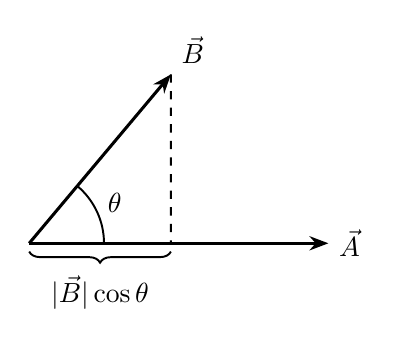
\begin{tikzpicture}[>={Stealth[length=2.4mm]}, line width=0.7pt]
  \coordinate (O) at (0,0);
  \coordinate (A) at (3.8,0);
  \coordinate (B) at (50:2.8);
  \coordinate (P) at (1.8,0); % |B|cos(theta) ~ 2.8*0.643
  \draw[->, line width=1.1pt] (O)--(A) node[right]{$\vec A$};
  \draw[->, line width=1.1pt] (O)--(B) node[above right]{$\vec B$};
  \draw[dashed] (B)--(P);
  \draw (0.95,0) arc (0:50:0.95); \node at (25:1.2){$\theta$};
  \draw[decorate, decoration={brace, mirror, raise=3pt, amplitude=4pt}] (O)--(P)
        node[midway, below=8pt]{$|\vec B|\cos\theta$};
\end{tikzpicture}
\end{document}
